\documentclass{article}
\usepackage{graphicx}
\graphicspath{ {./} }
\usepackage[margin=0.75in]{geometry}

\title{SCAJoop Final Project}
\author{
	Surekha Jadhwani\\
	\texttt{jadhwani.s@husky.neu.edu}
	\and 
	Joseph Sackett\\
	\texttt{joseph@sackett.com}
	\and 
	Akash Singh\\
	\texttt{singh.aka@husky.neu.edu}
	\and
	Christopher Willig\\
	\texttt{willig.c@husky.neu.edu}
}
\date{April 22 2016}
\begin{document}
 \maketitle
\textbf{Overview} \\ 
This project involved building a MapReduce framework to run arbitrary jobs. Our goal was to take a working Hadoop job, change only the import statements, compile it against our SCAJoop framework, and run it on a cluster of AWS EC2 machines.\\

\textbf{Architecture} \\
The SCAJoop architecture borrows ideas from Hadoop. The Job Runner uses the distribution framework to communicate with the Node Managers on each machine. The same general distribution framework is used for assignment A9 to start arbitrary tasks on the remote machines. SCAJoop is built on top of this distribution framework but, in this case, it can run arbitrary user mappers and reducer logic.\\
Below is the Architecture Diagram:\\

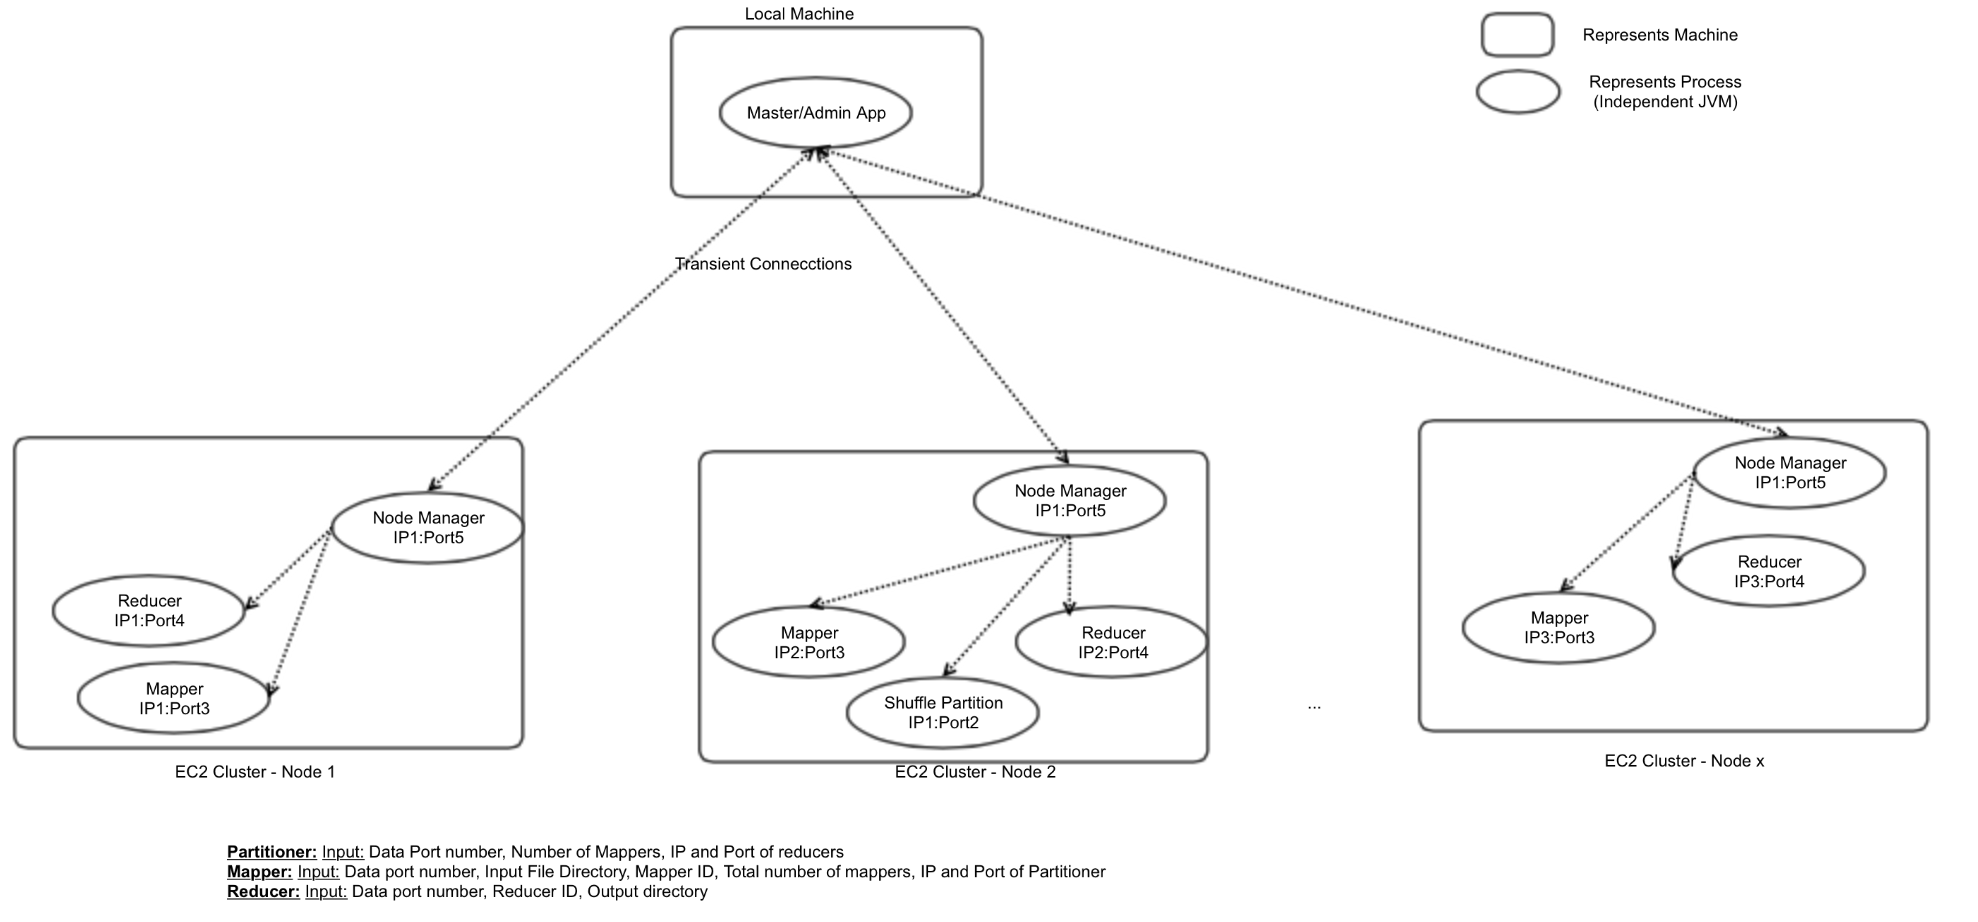
\includegraphics[width=16.5cm,height=10cm]{SCAJoopArch.png}
\bigskip

\textbf{Design} \\
The SCAJoop framework provides an API that user jobs target in order to run their distributed MapReduce job. The class structure is completely modeled after Hadoop. Every class in the client-side framework (the classes that the user program extends, implements, etc.) has an equivalent in the Hadoop framework. Our philosophy is that the programmer can port their code seamlessly between Hadoop and SCAJoop, changing only the import statements.\\ Most of the classes are simply stubs or POJOs to maintain class/interface relationships but the two most important classes are the Job and ToolRunner classes. The ToolRunner class is important because it creates a configuration object, reads in the configuration file (cluster\_conf), and then calls the user program's run() function. The Job class is very similar to the Admin class from A9. It's more-or-less the same except that there is no shell. The waitForCompletion() function is arguably the most important function in those two classes. This function does the "heavy lifting" from the client-side point of view. It will create a cluster (either local or AWS), submit the job to that cluster, block, and output log messages to the user console until all of the cluster reducers stop running, at which point the user program exits. \\
MapperTask is a generic class which is parameterized with the user’s Mapper class. The input files come from the specified input directory, which can be a local directory or AWS S3 bucket. Each mapper task is given an Id number and total number of mappers, which is used to distribute equal number of independent files to each mapper. For each file, it reads and separates input lines into the key and value. The MapperTask then delegates this key/value tuple to the user’s Mapper logic, passing a context for use in writing Mapper output in order to send to the Partitioner.\\
The design of the Partitioner deviates from Hadoop. We decided that it should only perform partitioning and the sorting would be moved to the reducers. This prevents the use of a secondary sort but distributing the sorting logic to separate machines provides some performance benefits. The role of the Partitioner is to simply take the hash code of the key modulo the number of reducers and forward the tuple there. \\
As with MapperTask, ReducerTask is a generic class which is parameterized with the user’s Reducer logic. We innovated the ReducerTask, eliminating the sorting stage in our implementation and added multi-threaded reduce support. After receiving keys and values from the Partitioner, the keys and values are stored in a HashMap. The HashMap contains different keys and ArrayLists of values associated with the keys. After the build up of the HashMap, reduce is called in a multithreaded mode working at a time on up to six keys. If there are more than six keys, only unto six are processed at a time as a batch and then the rest are reduced by unto six at a time batch method. The value of six can be changed via the variable to alter the number of threads being run at a time. These are couple of optimizations allow the user job to be efficiently reduced.\\

\textbf{Results} \\
Our testing involved converting our original A2 to run on SCAJoop. We executed the job and compared the results. These tied out to the Hadoop version and the A2 generated graph is displayed at the end of this document. \\
Comparative performance results listed below for the same data set (25 files):
\par
\bigskip
\begin{tabular}{| l | r |}
   & Run Time \\
  SCAJoop (5 * t2.large) & 1:30  \\
  Hadoop Pseudo & 2:50 \\
  AWS EMR  (3 * m3.xLarge) & 2:40 \\
\end{tabular}\\
\bigskip

\textbf{}\\   
\textbf{Limitations} \\
The most significant limitation is that SCAJoop only handles Text data types. It does not yet handle other Hadoop Writable data types. It would be a natural extension to handle these and transfer between nodes via serialization. As mentioned earlier, the Partitioner does not perform the shuffle and sort as does Hadoop. This curtails any secondary sort capability and limits the flexibility offered by the complex keys, comparators, and custom partitioners. There is also not yet any support for InputFormatters so the default key/value implementation goes to the Mapper.\\

\textbf{Summary} \\
Our final project achieved the goals we set. A simple, existing Hadoop job can be compiled and run, unchanged, against SCAJoop. We tested this and the results tied out. Our distribution framework, controlled by the JobRunner can theoretically scale to any number of machines. This was an educational and successful project.\\
Akash was the architect and developer of Mapper and Reducer. Joe built the general frameworks for distribution and SCAJoop jobs, as well as the Partitioner. Chris built the JobRunner, its peer NodeManagers, as well as the image spawned on each EC2 node. Surekha developed much of the MapperTask and ReducerTask code and tied everything together to get it working. These were good results, accomplished by hard work from everyone on the team. 

\bigskip
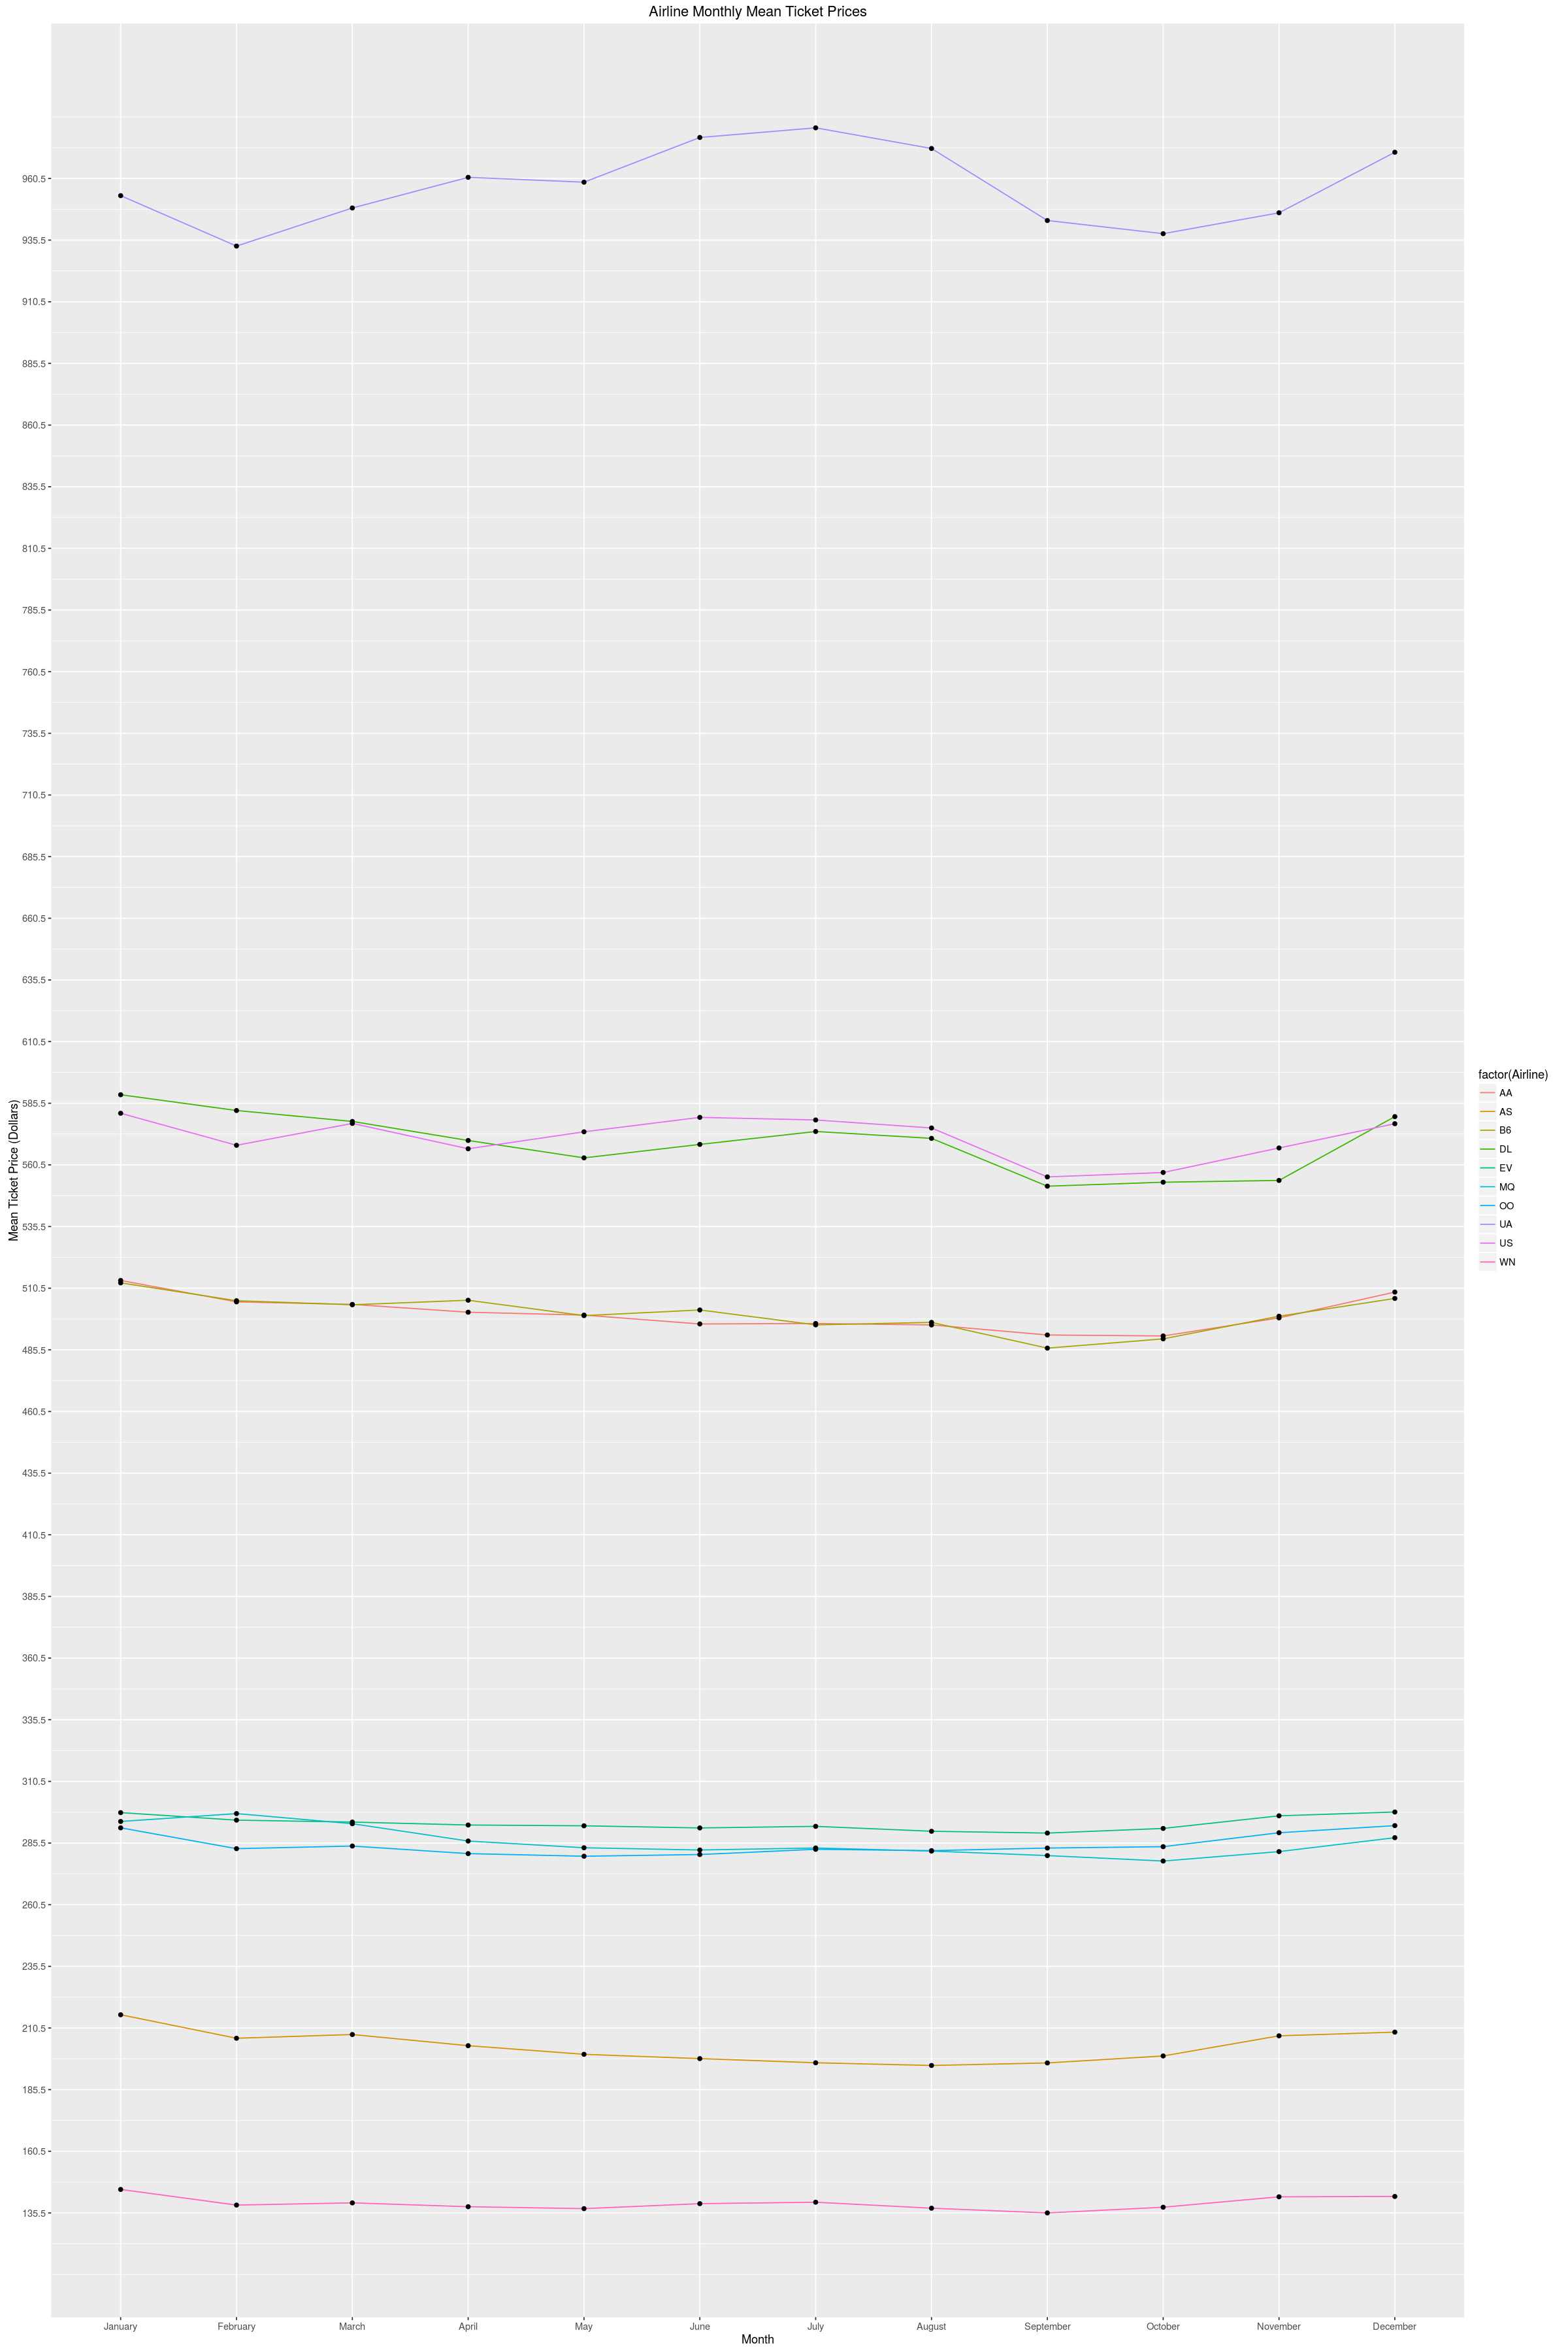
\includegraphics[height=20cm,width=16.25cm]{plot.png}

\end{document}
